\documentclass[a4paper,12pt]{article}

\usepackage[T2A]{fontenc}
\usepackage[utf8x]{inputenc}
\usepackage[russian,english]{babel}
\usepackage{graphicx}
\usepackage{color}
\usepackage{xcolor}
\usepackage{listings}
\usepackage{fancyhdr}
\usepackage{amsmath}
\usepackage{indentfirst} % включить отступ у первого абзаца
\usepackage{url}
\usepackage{supertabular}
\usepackage{hhline}
\usepackage{semantic}

%%\usepackage[
%%		a4paper, includefoot,
%%		left=3cm, right=1cm, top=2cm, bottom=1.5cm,
%%		headsep=1cm, footskip=1cm
%%	]{geometry}

\title{Лабораторная работа №4}
\author{Кузнецов Д.Б.\and Вагин Д.А.}
\date{11/2011}
\pagestyle{empty}
\pagestyle{fancy}
\lhead{Лабораторная работа №4} %верхний колонтитул слева

\lstloadlanguages{c++,html,sql,pascal,make,tex}
\lstset{
	language=html,inputencoding=utf8x,
	extendedchars=\true,captionpos=b,tabsize=4,
	frame=lines,
	keywordstyle=\color{blue},commentstyle=\color{green},stringstyle=\color{red},
	breaklines=true,showstringspaces=false,basicstyle=\footnotesize
}
\lstset{
	language=c++,inputencoding=utf8x,
	extendedchars=\true,captionpos=b,tabsize=4,
	frame=lines,
	keywordstyle=\color{blue},commentstyle=\color{green},stringstyle=\color{red},
	breaklines=true,showstringspaces=false,basicstyle=\footnotesize
}
\lstset{
	language=sql,inputencoding=utf8x,
	extendedchars=\true,captionpos=b,tabsize=4,
	frame=lines,
	keywordstyle=\color{blue},commentstyle=\color{green},stringstyle=\color{red},
	breaklines=true,showstringspaces=false,basicstyle=\footnotesize
}
\lstset{
	language=pascal,inputencoding=utf8x,
	extendedchars=\true,captionpos=b,tabsize=4,
	frame=lines,
	keywordstyle=\color{blue},commentstyle=\color{green},stringstyle=\color{red},
	breaklines=true,showstringspaces=false,basicstyle=\footnotesize
}
\lstset{
	language=make,inputencoding=utf8x,
	extendedchars=\true,captionpos=b,tabsize=4,
	frame=lines,
	keywordstyle=\color{blue},commentstyle=\color{green},stringstyle=\color{red},
	breaklines=true,showstringspaces=false,basicstyle=\footnotesize
}

\begin{document}

\paragraph{Построение синтаксического анализатора на основании LR грамматики}

\paragraph{Порядок выполнения}
\begin{enumerate}
	\item Построить грамматику с предшествованием
	\item Определить отношения предшествования
	\item Изобразить восходящую схему разбора
	\item Выполнить свертку заданного примера
	\item Разработать синтаксический анализатор на базе yacc
	\item Разработать лексический анализатор на базе lex
	\item Выполнить синтаксический анализ заданного примера
\end{enumerate}

\subparagraph{Состав отчета}
\begin{itemize}
	\item Титульный лист (фамилия, группа, номер варианта, наименование работы, задание)
\end{itemize}

\paragraph{Варианты заданий}
В задании указано содержательное описание грамматики и простейший пример для облегчения понимания.
\begin{enumerate}
	\item конструкция for языка с++. 
\begin{lstlisting}[language=c++,{caption=for}]
for(
	a=0, b=76; 
	i<10 && b>0 ;
	++i, b=i+1
){ 
	b++;
	i++;
}
\end{lstlisting}

	\item конструкция if языка c++. 
\begin{lstlisting}[language=c++,{caption=if}]
if(a==0 && b<=0)
{
	a=b; b++;
}
else
{
	a++; 
	b+=2;
}
\end{lstlisting}

	\item конструкция switch языка c++. 
\begin{lstlisting}[language=c++,{caption=switch}]
switch(a){ 
	case 1: a=1; 
	case 3: 
	case 2: a++; break; 
	default: a=0;
}
\end{lstlisting}

	\item тэг img языка разметки HTML: 
\begin{lstlisting}[language=html,{caption=img}]
<img src="/images/a.png" width="20" height="30" 
	alt="картинка" />
\end{lstlisting}

	\item Объявление функции в c++:
\begin{lstlisting}[language=c++,{caption=func}]
int funcname(int a, char b, float c = 0.1);
\end{lstlisting}

	\item тэг table языка разметки HTML: 
\begin{lstlisting}[language=html,{caption=table}]
<table>
	<tr>
		<th>заголовок 1</th>
		<th>заголовок 2</th>
	</tr>
	<tr>
		<td>ячейка 1</td>
		<td>ячейка 2</td>
	</tr>
	<tr>
		<td>ячейка 3</td>
		<td>ячейка 4</td>
	</tr>
</table>
\end{lstlisting}

	\item тэг ul (ненумерованный список) языка разметки HTML: 
\begin{lstlisting}[language=html,{caption=ul}]
<ul>
	<li>item 1</li>
	<li>item 2</li>
	<li>item 3</li>
</ul>
\end{lstlisting}

\item конструкция while языка c++. 
\begin{lstlisting}[language=c++,{caption=while}]
while( a>0 || b<76){
	b++;
	a++;
}
\end{lstlisting}

\item конструкция do-while языка c++. 
\begin{lstlisting}[language=c++,{caption=do-while}]
do{
	b++;
	a++;
}while( a>0 || b<76);
\end{lstlisting}

	\item конструкция insert языка запросов SQL:
\begin{lstlisting}[language=sql,{caption=insert}]
insert into tablename(pk,column1,column2) 
values (1, 2 , 'varchar');
\end{lstlisting}

	\item конструкция select языка запросов SQL:
\begin{lstlisting}[language=sql,{caption=select}]
select pk, column1, column2
from tablename
where column1 = 2 
	and column2 like 'xxx%';
\end{lstlisting}

	\item конструкция delete языка запросов SQL:
\begin{lstlisting}[language=sql,{caption=delete}]
delete from tablename
where column1 = 1
	or column2 like 'xxx%';
\end{lstlisting}

	\item тэг form языка разметки HTML: 
\begin{lstlisting}[language=html,{caption=form}]
<form methid="post" action="/registration/">
	<input type="text" name="login" />
	<input type="text" name="email" />
	<input type="password" name="password" />
	<input type="submit"/>
</form>
\end{lstlisting}

	\item конструкция if языка Pascal: 
\begin{lstlisting}[language=pascal,{caption=if}]
if (a <= 10) or (b >= 2) then
begin
	a := 10;
	b := 10;
end else
	a := b;

\end{lstlisting}

	\item конструкция for языка Pascal: 
\begin{lstlisting}[language=pascal,{caption=for}]
for i:= 0 to 10 step 2 do 
begin
	a := i;
end;
\end{lstlisting}

\end{enumerate}

\paragraph{Пример реализации}
Построим грамматику \\
$S -> sXfX$\\
$X -> xY$\\
$X -> x$\\
$Y -> ,xY$\\
$Y -> ,x$\\

\begin{tabular}[l]{c|cccccc}
    & $s$ & $X$ & $Y$ & $x$ & $f$ & $,$ \\
\hline
$s$ &     & $=$ &     & $<$ &     &     \\
$X$ &     &     &     &     & $=$ &     \\
$Y$ &     &     &     &     & $>$ &     \\
$x$ &     &     & $=$ &     & $>$ & $<$ \\
$f$ &     & $=$ &     & $<$ &     &     \\
$,$ &     &     &     & $=$ &     &     \\
\end{tabular}

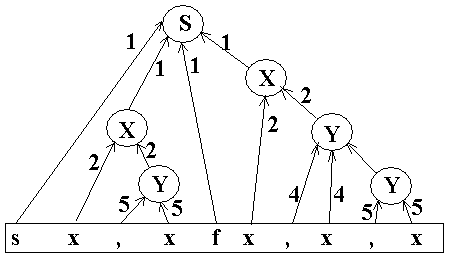
\includegraphics[scale=1.0]{lab4.png}\vspace{1em}

Обозначим условно \textasciicircum как начало, а \$ как конец строки.\\
\begin{math}
sx,xfx => \\
<s<x<, \doteq x>f<x> => \\
<s<x \doteq Y>f \doteq X> => \\
<s<X \doteq f \doteq >X> => <S>
\end{math}\\

\begin{lstlisting}[language=tex,{caption=lab4.l}]
%%
x               { return x; }
f               { return f; }
,               { return comma; }
.               { return yytext; }
%%
\end{lstlisting}

\begin{lstlisting}[language=tex,{caption=lab4.y}]
%start start

%token f x comma

%%

start:  X f X { printf("%s\n", "OK");}
        ;
X :     x
        | x Y
        ;
Y :     comma x
        | comma x Y
        ;

%%
/* start of programs */
#include "lex.yy.c"

main() { return  yyparse();}

yyerror(char *s) { fprintf(stderr,"%s\n",s); }
\end{lstlisting}

Выполняем в shell следующие комманды:
\begin{verbatim}
flex lab4.l
yacc lab4.y
gcc -o lab4 y.tab.c -ll
./lab4
\end{verbatim}

\end{document}
